
% THIS IS AN EXAMPLE DOCUMENT FOR VLDB 2012
% based on ACM SIGPROC-SP.TEX VERSION 2.7
% Modified by  Gerald Weber <gerald@cs.auckland.ac.nz>
% Removed the requirement to include *bbl file in here. (AhmetSacan, Sep2012)
% Fixed the equation on page 3 to prevent line overflow. (AhmetSacan, Sep2012)


\section{Introduction}
\label{sec:intro}
Combining human computation with traditional computation has been recently proven beneficial in extracting knowledge and acquiring data for many application domains, including recommendation systems~\cite{amsterdamer:2014}, knowledge base completion~\cite{kondredi:2014}, entity extraction and structured data collection~\cite{trushkowsky:2013, park:2014}. In fact, extracting information, and entities in particular, from the crowd has been shown to provide access to more fine grained information that may belong to the long tail of the web or even be completely unavailable on the web~\cite{franklin:2011, Parameswaran:2012, west:2014}.

A fundamental challenge in crowdsourced entity extraction is reasoning about the completeness of the extracted information. More precisely, given a task that seeks to enumerate entities from a specific domain by asking human workers, e.g., extract all restaurants in New York, it is not easy to judge if we have extracted all entities (in this case restaurants). This is because we are in an ``open world"~\cite{franklin:2011} scenario. 

Recent work~\cite{trushkowsky:2013} has considered the problem of crowdsourced entity extraction using a single type of {\em query} that is asked to humans; for our restaurant case, the query will be ``give me another restaurant in New York''. That paper determines how many times this query must be asked to different human workers before we are sure we have extracted all restaurants in New York. However, given the latency and monetary cost inherent in leveraging crowdsourcing, it is easy to see that just using this query repeatedly will not be practical for real-world applications, for two coupled reasons: (a) {\em wasted cost:} we will keep receiving the most popular restaurants and will have to wait a long while before we receive new or unseen restaurants (b) {\em lack of coverage:}  beyond a point all the restaurants we get will already be in our set of extracted entities --- thus, for the less popular restaurants, we may never end up receiving them at all.


% Extracting entities from the crowd can be done by issuing {\em queries} of the form ``Give me $k$ entities corresponding to a specific domain". In our restaurant example, such queries may correspond to crowdsourced task of the form ``give me 5 French restaurant in Manhattan, NY". Recent work has considered this problem for isolated queries~\cite{trushkowsky:2013} , i.e., queries that correspond to exactly the same question and are repeatedly evaluated against workers. In this line of work, the query predicates specify the data domain of interest. 

In this paper, our goal is to {\em make crowdsourced entity extraction practical}. To do so, we leverage a structured entity domain, i.e., a domain that can be fully described by a collection of attributes, each potentially displaying hierarchical structure. For example, in our restaurant case, we could have one attribute about location, one about cuisine, and one about whether the restaurant does takeout. We can then leverage this entity domain to use a much richer space of queries asked to human workers, considering all combinations of values for each of these attributes, e.g., ``give me another Moroccan restaurant in Manhattan, New York, that does takeout".  In this manner, we can leverage these {\em specific, targeted queries} to extract not-so popular entities with attribute values set to specific ones, e.g., in this case, cuisine is Moroccan, location is Manhattan, and takeout is Yes.

If we view the structured data domain as a lattice, then each query can be mapped to a node in this lattice. Thus, our goal is to traverse this lattice by issuing queries corresponding to various nodes in this lattice, often multiple times at each node. However, this lattice can be often large, leading to a host of additional challenges in deciding which queries to issue at any point: (a) {\em Sparsity:} Many of the nodes in the lattice are likely to be empty, i.e., the queries corresponding to those nodes are likely to not have any answers; avoiding asking queries corresponding to these nodes is essential to keep monetary cost low. (b) {\em Interrelationships:} Many of the nodes in the lattice are ``coupled'' with one another; for example, the results from a few queries corresponding to ``give me another Moroccan restaurant in Manhattan, New York'' can inform whether issuing queries corresponding to ``give me another Moroccan restaurant in Manhattan, New York, that does takeout'' is useful or not. Unfortunately, the techniques from Trushkowsky et al.~\cite{trushkowsky:2013} do not directly apply to the scenario where we are traversing a lattice corresponding to this structured data domain, and new techniques are needed. Furthermore, unlike Trushkowsky et al.~\cite{trushkowsky:2013}, we focus on the budgeted case, where we are given a budget and we want to maximize the number of retrieved entities; we believe this is a more practical goal, instead of the goal of retrieving all entities. We describe additional challenges in detail in Section~\ref{sec:challenges}.

Our crowdsourced entity extraction techniques can be useful for a variety of applications that are naturally coupled to a structured entity domain, including:
\squishlist
\item A newspaper that wants to collect a list of today's events to be displayed on the events page every day. 
In this case, the structured data domain could include event type (e.g., music concerts vs.~political rallies) or location, among other attributes.
\item A stock trading firm wants to collect a list of stocks that have been mentioned by popular press on the previous day. In this case, the structured data domain could include stock type, popular press article type, or whether the mention was positive or negative, among other attributes. 
\item A real estate expert wants to curate a list of houses available for viewing today. 
\item XXX: a couple more would be good
\squishend





% Often, however, crowd entity extraction techniques are used to acquire information from large data domains that cannot be described adequately by a single query with fixed predicates. Consider for example a scenario where crowd sourcing techniques are used to collect information about various types of events (e.g., music concerts or political rallies) over different countries. If we just asked workers to provide us with events without specifying the event type or location, we would get a limited number of {\em popular} events. Moreover, the characteristics of collected events would heavily depend on the demographics of the workers completing the task. For example, a US based worker is more likely to provide us with events occurring in the state she is located. 

% However, if we want to maximize the number of extracted events we can intuitively issue multiple diversified queries, requesting the crowd to provide information for specific types of events potentially focusing on a specific location. Notice, that following this approach we are less likely to be affected by heavily popular events and the worker specific characteristics. However, deciding on the right queries in such domains entails several challenges. Next, we use a real-world scenario to illustrate these challenges.

\subsection{Challenges and Opportunities}
\label{sec:challenges}
We consider Eventbrite~\footnote{https://www.eventbrite.com}, an online event aggregator, that relies on crowdsourcing to compile a directory of events with detailed information about the location, type, date and category of each event. Typically, event aggregators are interested in collecting information about diverse events spanning from conferences and music festivals to political rallies for multiple locations across different location, i.e., countries or cities. In particular, Eventbrite collects information about events across different countries in the world. Each country is further split into cities and areas across the country. Moreover, events are organized according to their type and topic. We collected a dataset from Eventbrite spanning over 63 countries that are divided into 1,709 subareas (e.g., states) and 10,739 cities, containing events of 19 different types, such as rallies, tournaments, conferences, conventions, etc. and a time period of 31 days spanning over the months of October and November. It is easy to see that two of the three dimensions, i.e., location and time, describing the domain of collected events  are hierarchically structured. The overall domain can be fully specified if we consider the cross product across the possible values for location, event type and time. For each of the location, time, type dimensions we also consider a special {\em wildcard} value. Taking the cross-product across the possible values of these dimensions results in a total of 8,508,160 points containing 57,805 distinct events overall.

The first challenge stems from the fact that due to the sheer size of the data domain there are potentially many sparsely populated points, i.e., points  that contain only a limited number of items. Assuming a given budget for crowdsourced entity extraction, one needs to avoid such points when issuing crowdsourced entity enumeration queries in order to maximize the number of extracted entities under the specified budget. 

\begin{example}
We focus on the collected Eventbrite dataset and plot the number of items for each of the data items associated the event domain under consideration. Out of 8,508,160 points only 175,068 points are associated with events while the remaining points have zero events. \Cref{fig:eventbritepop} shows the number of events associated with these point. Notice that the y-axis is in log-scale. As shown the majority of populated points have less than 100 items. It is obvious that when trying to extract events from such a sparse domain one needs to optimize the crowdsourced queries if operating under a monetary budget.
\end{example}

\begin{figure}
	\begin{center}
	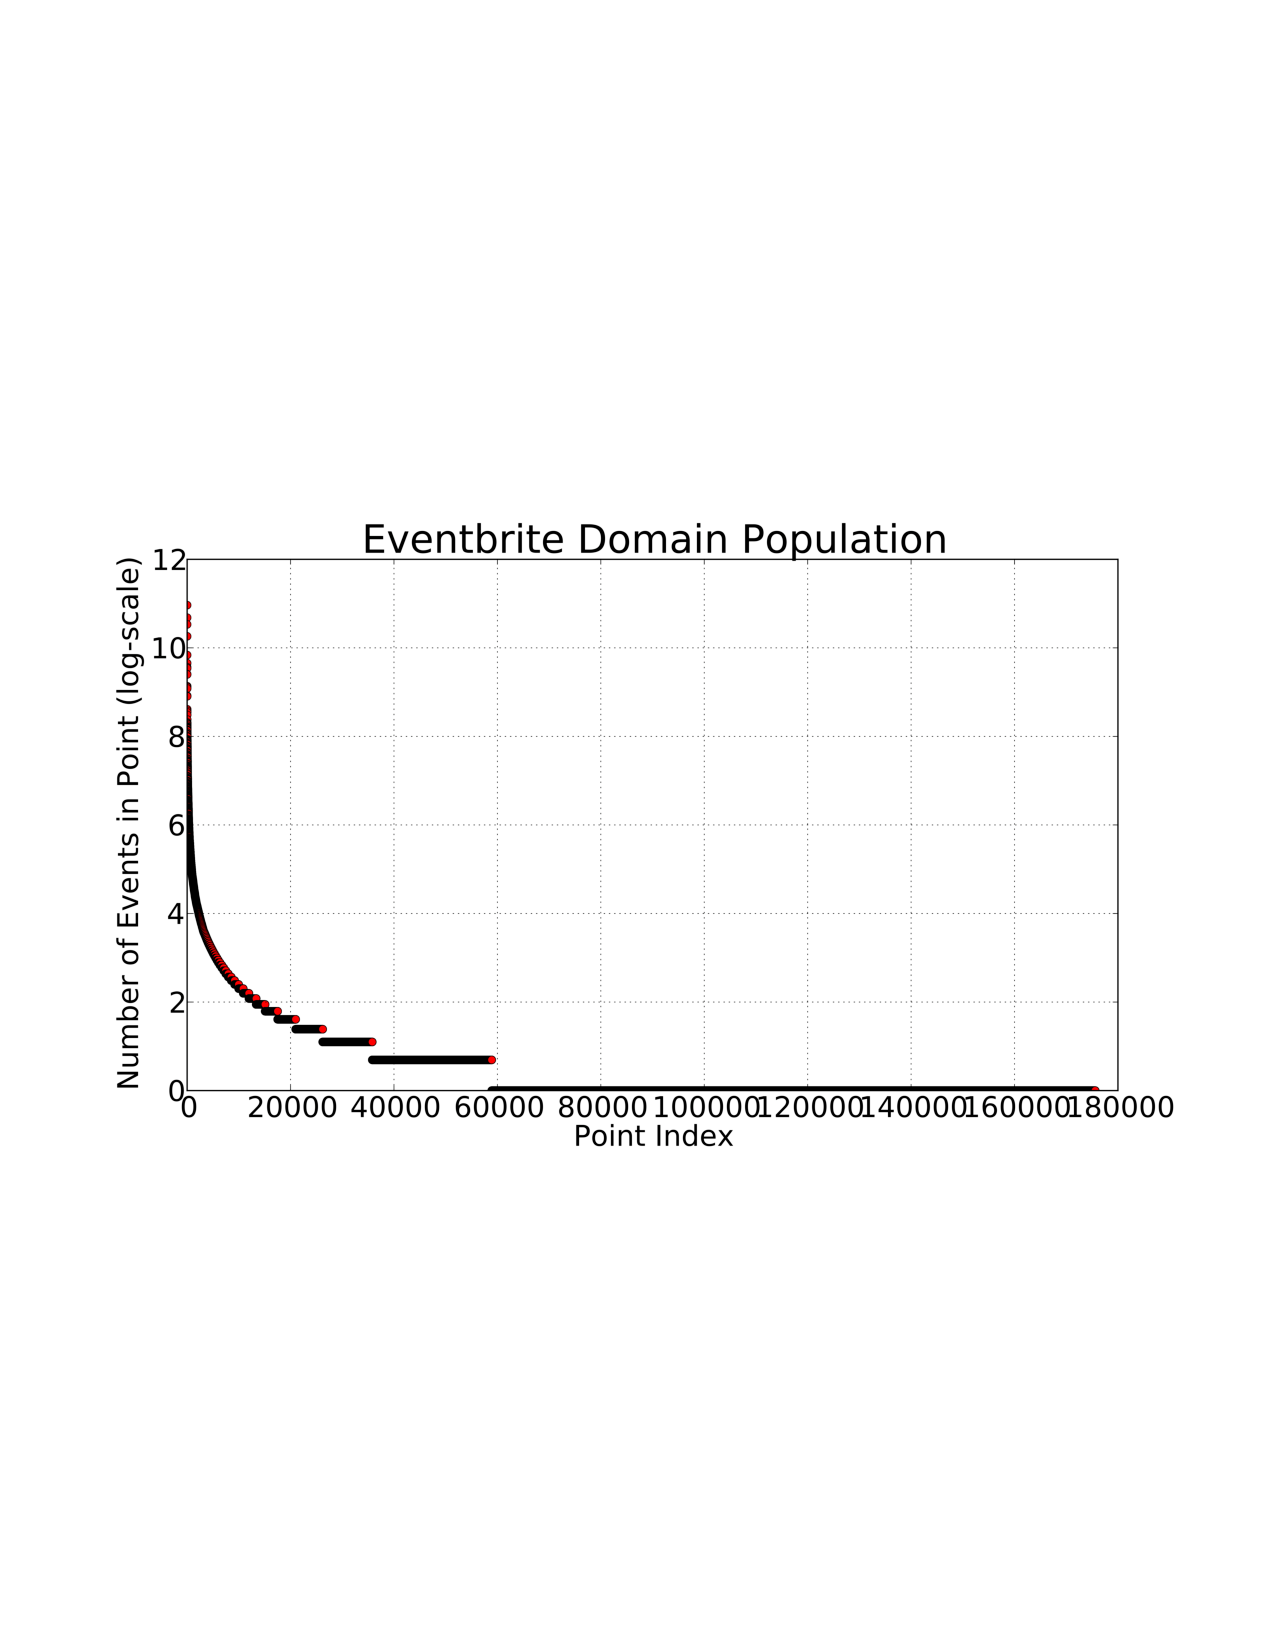
\includegraphics[trim=55 240 40 250,clip,scale=0.4]{figs/eventBritePopulationSS.pdf}
	\caption{The attributes describing the events domain and the hierarchical structure of each attribute.}
	\label{fig:eventbritepop}
	\vspace{-20pt}
	\end{center}
\end{figure}

However, the hierarchical structure of the data domain presents us with an opportunity. In fact, we observe that the heavily populated domain points are not {\em leaf points}, i.e., points for which all the dimension values are specified but points for which one or more dimensions are assigned the wildcard value and thus can obtain any value. In fact, one can exploit this to maximize the number of extracted entities as we further discuss in \Cref{sec:prelims}.

The second challenge when consider large domains such as the Eventbrite domain, is the overlaps among different points of the domain. More precisely, when we ask the crowd to provide us with entities associated with a domain specific point (e.g., events in New York) these entities may be associated with other points in the domain (e.g., concerts in New York). Therefore we indirectly obtain information about the population of domain points for which no queries may have been issues. 
These dependencies across queries pose a significant challenge when estimating the number of new entities obtain by a query.

\begin{example}
We consider again the Eventbrite dataset and plot the pairwise overlaps of the ten most populous points in the domain. \Cref{fig:eventbriteover} shows the Jackard index for the corresponding point pairs. As shown the event populations corresponding to these points overlap significantly. It is easy to see that when issuing queries at a certain domain point, we not only obtain events corresponding to this point but to other points in the domain as well. 
\end{example}

\begin{figure}
	\begin{center}
	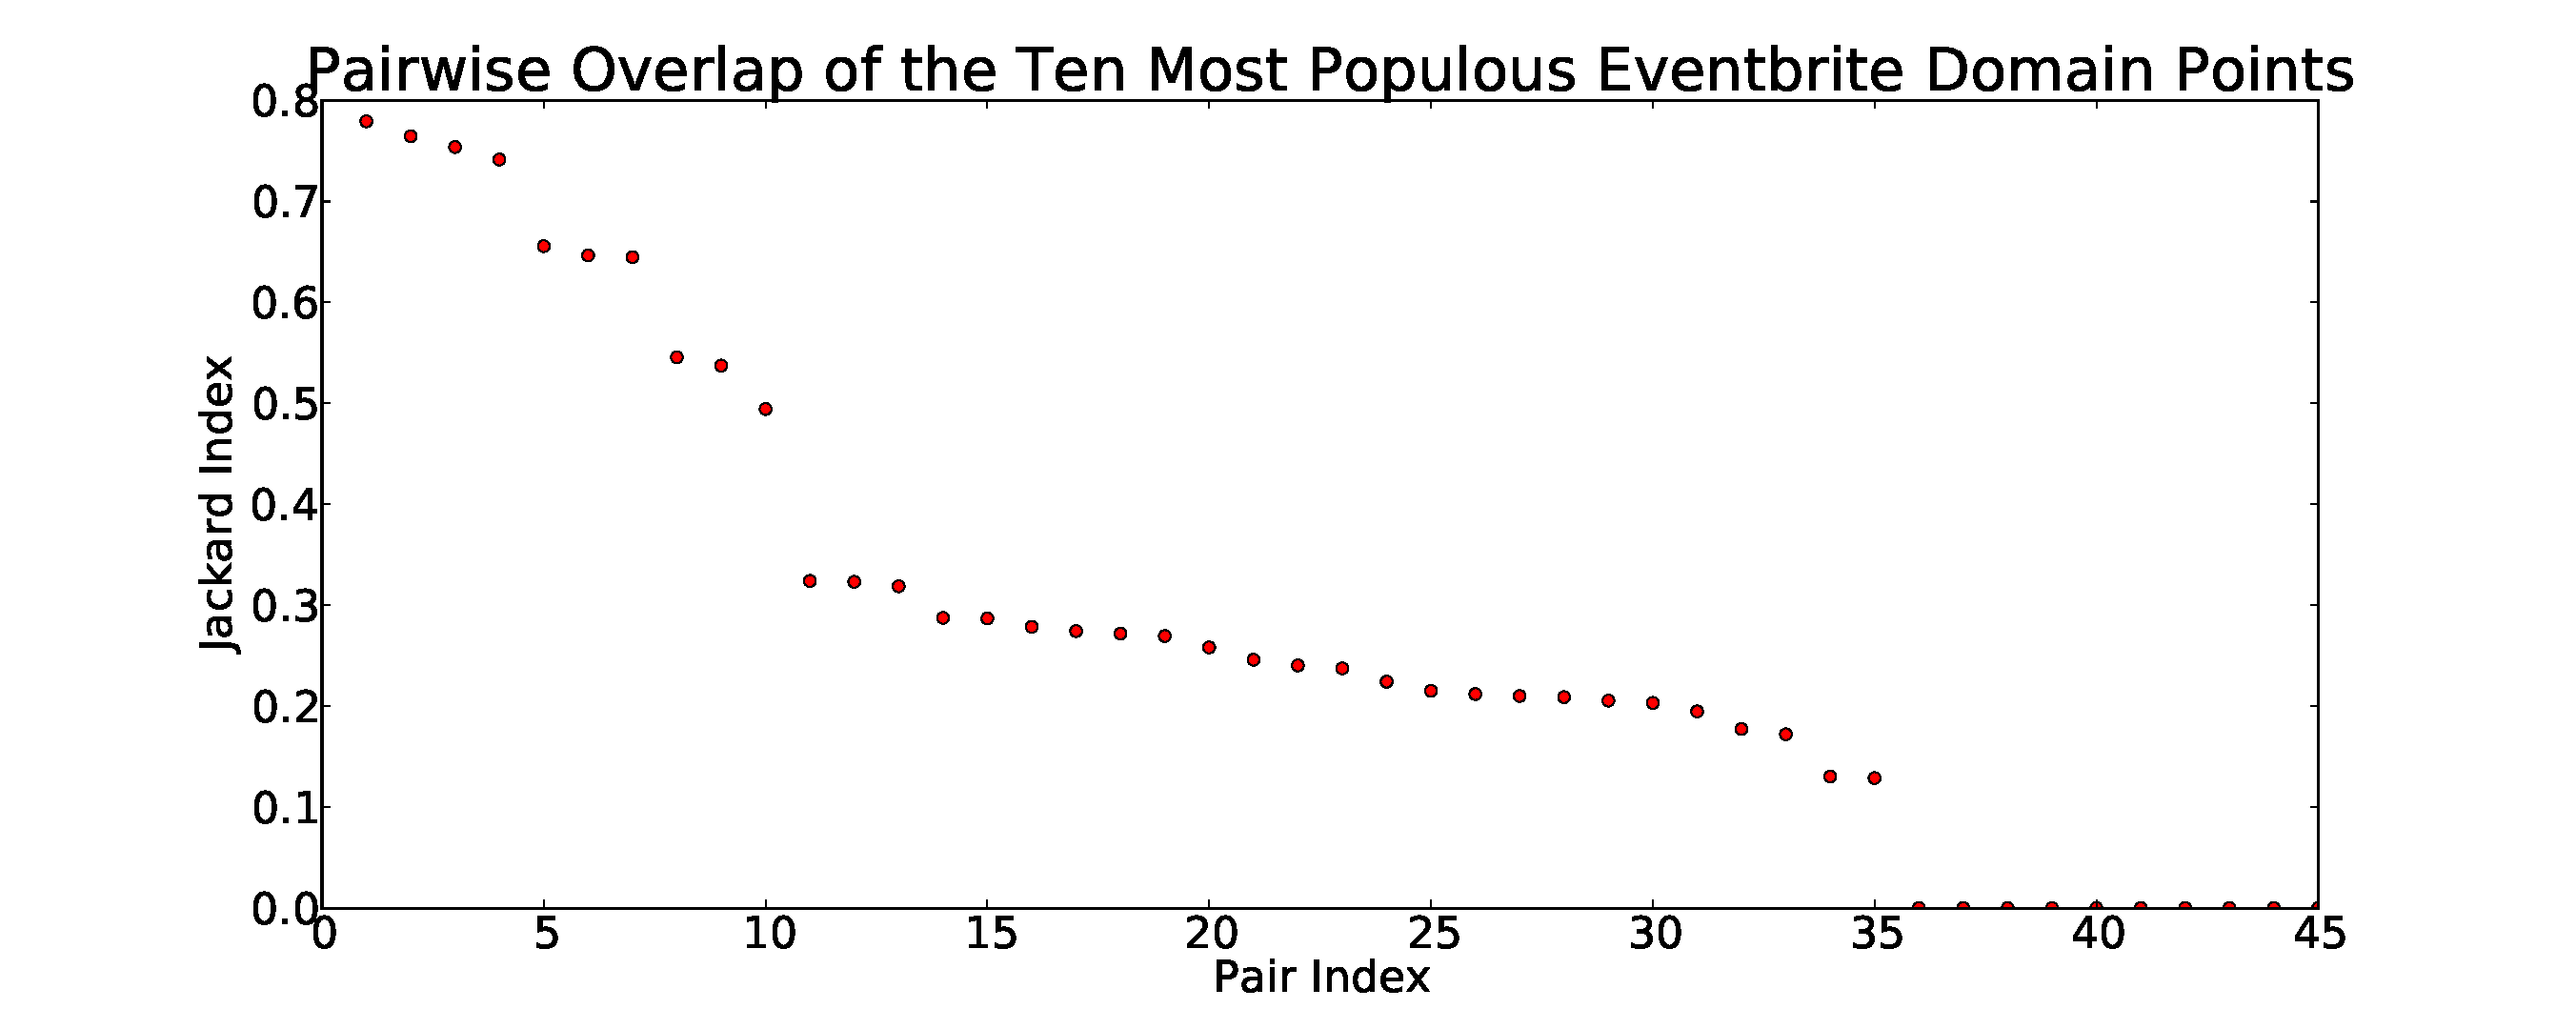
\includegraphics[trim=55 0 62 0,clip,scale=0.2]{figs/overlaps.pdf}
	\caption{Pairwise overlaps of the 10 most populous domain points in Eventbrite.}
	\label{fig:eventbriteover}
	\vspace{-20pt}
	\end{center}
\end{figure}

\subsection{Contributions}
\label{sec:contributions}
Motivated by these examples, we study the problem of {\em budgeted crowd entity extraction} over {\em structured domains}. More precisely, we focus on domains described by a collection of attributes, each following a known {\em hierarchical structure}, i.e., we assume that for each attribute the corresponding hierarchy is known.

We propose a novel algorithmic framework that exploits the structure of the domain to maximize the number of extracted entities under given budget constraints. In particular, we view the problem of entity extraction as a {\em multi-round adaptive optimization problem}. At  each round we exploit the information on extracted entities obtained by previous queries to adaptively select the crowd query that will maximize the {\em gain} and cost trade-off at each round. The gain of a query is defined as the number of new unique entities extracted by it. We extend on previous query interfaces that considered only questions of the type ``Give me $k$ more entities" and examine {\em generalized queries} that can also include an {\em exclude list}. In general such queries are of the type ``Give me $k$ more entities that are not $A$, $B$, etc". Building upon techniques from the species estimation and the multi-armed bandits literature, we introduce a new methodology for estimating the gain for such generalized queries and show how the hierarchical structure of the domain can be exploited to improve the accuracy of our gain estimates. Our main contributions are as follows:

\squishlist
\item We study the challenge of information flow across entity extraction queries for overlapping parts of the data domain.
\item We develop a new technique to estimate the gain of generalized entity extraction queries under the presence of dependent information. The proposed technique exploits the structure of the data domain to obtain accurate estimates. 
\item We introduce an adaptive optimization algorithm that takes as input the gain estimates for different types of queries and identifies querying policies that maximize the total number of retrieved entities under given budget constraints. 
\item Finally, we show that our techniques can effectively solve the problem of budgeted crowd entity extraction for large data domains on both real-world and synthetic data.
\squishend

